\documentclass[11pt,a4paper]{article}
%%%%%%%%%%%%%%%%%%%%%%%%% Credit %%%%%%%%%%%%%%%%%%%%%%%%

% template ini dibuat oleh martin.manullang@if.itera.ac.id untuk dipergunakan oleh seluruh sivitas akademik itera.

%%%%%%%%%%%%%%%%%%%%%%%%% PACKAGE starts HERE %%%%%%%%%%%%%%%%%%%%%%%%
\usepackage{graphicx}
\usepackage{caption}
\usepackage{microtype}
\captionsetup[table]{name=Tab.}
\captionsetup[figure]{name=Obr.}
\usepackage{tabulary}
%\usepackage{minted}
% \usepackage{amsmath}
\usepackage{fancyhdr}
% \usepackage{amssymb}
% \usepackage{amsthm}
\usepackage{placeins}
% \usepackage{amsfonts}
\usepackage{graphicx}
\usepackage[all]{xy}
\usepackage{tikz}
\usepackage{verbatim}
\usepackage[left=2cm,right=2cm,top=3cm,bottom=2.5cm]{geometry}
\usepackage{hyperref}
\hypersetup{
	colorlinks,
	linkcolor={red!50!black},
	citecolor={blue!50!black},
	urlcolor={blue!80!black}
}
\usepackage{caption}
\usepackage{subcaption}
\usepackage{multirow}
\usepackage{psfrag}
\usepackage[T1]{fontenc}
\usepackage[scaled]{beramono}
% Enable inserting code into the document
\usepackage{listings}
\usepackage{xcolor} 
% custom color & style for listing
\definecolor{codegreen}{rgb}{0,0.6,0}
\definecolor{codegray}{rgb}{0.5,0.5,0.5}
\definecolor{codepurple}{rgb}{0.58,0,0.82}
\definecolor{backcolour}{rgb}{0.95,0.95,0.92}
\definecolor{LightGray}{gray}{0.9}
\lstdefinestyle{mystyle}{
	backgroundcolor=\color{backcolour},   
	commentstyle=\color{green},
	keywordstyle=\color{codegreen},
	numberstyle=\tiny\color{codegray},
	stringstyle=\color{codepurple},
	basicstyle=\ttfamily\footnotesize,
	breakatwhitespace=false,         
	breaklines=true,                 
	captionpos=b,                    
	keepspaces=true,                 
	numbers=left,                    
	numbersep=5pt,                  
	showspaces=false,                
	showstringspaces=false,
	showtabs=false,                  
	tabsize=2
}
\lstset{style=mystyle}
\renewcommand{\lstlistingname}{Kode}
%%%%%%%%%%%%%%%%%%%%%%%%% PACKAGE ends HERE %%%%%%%%%%%%%%%%%%%%%%%%


%%%%%%%%%%%%%%%%%%%%%%%%% Data Diri %%%%%%%%%%%%%%%%%%%%%%%%
\newcommand{\student}{\textbf{Zajan Ondřej}}
\newcommand{\course}{\textbf{Virtuální instrumentace}}
%\newcommand{\assignment}{\textbf{xxx}}

%%%%%%%%%%%%%%%%%%% using theorem style %%%%%%%%%%%%%%%%%%%%
\newtheorem{thm}{Theorem}
\newtheorem{lem}[thm]{Lemma}
\newtheorem{defn}[thm]{Definition}
\newtheorem{exa}[thm]{Example}
\newtheorem{rem}[thm]{Remark}
\newtheorem{coro}[thm]{Corollary}
\newtheorem{quest}{Question}[section]
%%%%%%%%%%%%%%%%%%%%%%%%%%%%%%%%%%%%%%%%
\usepackage{lipsum}%% a garbage package you don't need except to create examples.
\usepackage{fancyhdr}
\pagestyle{fancy}
\fancyhf{}
\chead{Virtuální instrumentace}
\cfoot{\thepage}
\renewcommand{\headrulewidth}{0.4pt}
\renewcommand{\footrulewidth}{0.4pt}

%%%%%%%%%%%%%%  Shortcut for usual set of numbers  %%%%%%%%%%%

\newcommand{\N}{\mathbb{N}}
\newcommand{\Z}{\mathbb{Z}}
\newcommand{\Q}{\mathbb{Q}}
\newcommand{\R}{\mathbb{R}}
\newcommand{\C}{\mathbb{C}}
\setlength\headheight{14pt}

\renewcommand{\refname}{Reference}
\pagenumbering{arabic}  % číslování stránek čísly
%%%%%%%%%%%%%%%%%%%%%%%%%%%%%%%%%%%%%%%%%%%%%%%%%%%%%%%555
\begin{document}
	%\begin{flushright}
	%	\textbf{Zajan Ondřej\\ Brož Petr} \hspace{3.2cm} 
	%\end{flushright}
	\begin{center}
		\section*{\centering{Semestrální práce - Chytrý květináč - dokumentace\\Zajan Ondřej}}
	\end{center}

	
	\noindent
	\rule{17cm}{0.05cm}
	%%%%%%%%%%%%%%%%%%%%%%%%%%%%%%%%%%%%%%%%%%%%% BODY DOCUMENT %%%%%%%%%%%%%%%%%%%%%%%%%%%%%%%%%%%%%%%%%%%%%
	\section{Úvod}
	Můj projekt je tvořen třemi částmi: firmwarem procesoru, počítačovou aplikací a samotným hardwarem. Jeho srdcem je vývojová deska F3 Discovery s STM32, ke které jsou připojeny periférie květináče. Pro ovládání květináče uživatelovi slouží počítačová aplikace. Jednotlivé části jsou rozebrány dále.
	
	\section{Firmware}
	Firmware jsem vyvíjel v prostředí Cube IDE. Procesor slouží ke čtení: hladiny vody v misce, hladiny vody v rezervoáru, vlhkosti hlíny, vlhkosti vzduchu, teploty vzduchu. Procesor má následující výstupy: ovládání čerpadla, ovládání žárovky, ukládání na SD kartu, signalizační led diody umístěné přímo na vývojové desce, zapínání napájení květináče, komunikace přes sériovou linku.
	
	Příjem dat přes sériovou linku probíhá pomocí callbacků, kde se přijatá data ukládají do bufferu. Uvnitř hlavní programové smyčky pak pravidelně volám funkci, která v naskládaných datech hledá řádky a první řádek, který najde, uloží do proměnné $RXLine$, s kterou dále v programu pracuji. 
	
	V hlavní programové smyčce nejdříve čekám na přijetí aktuálního času z počítače. Procesor umožňuje využít interní časovač jako zdroj reálného času. Po nastavení datumu a času se ptám, zda nepřišly data ze sériové linky a zkoumám, zda nepřišel známý příkaz či známý datový balík. Datové balíky (pakety) posílám ve formátu "\{data1;data2;..\}" oběma směry. 
	
	Květináč má implementovány následující komunikační funkce:
	\begin{itemize}
		\item \textbf{getdata} - vytáhne data z květináče ve formátu:\\ "$\{temperature;humidity;watter\_cup;watter\_rez;soil1;soil2\}\backslash n\backslash r$", kde $temperature$ je aktuální teplota, $humidity$ je aktuální vlhkost vzduchu, $watter\_cup$ je aktuální hladina vody v misce, $watter\_rez$ je aktuální hladina vody v rezervoáru, $soil1$ je vlhkost půdy z prvního senzoru a $soil2$ je vlhkost půdy z druhého senzoru
		\item \textbf{getconfig} - vytáhne aktuální nastavení květináče ve formátu: "$\{mode;temperature;humidity\}\backslash n\backslash r$", kde $mode$ je aktuální režim zalévání, $temperature$ je teplota, která je udržována v kopuli, $humidity$ je vlhkost půdy, která je udržována (neimplementováno)
		\item \textbf{getstatus} - vytáhne z květináče aktuální stav řízení zalévání, ohřívání (ano/ne) ve formátu "$\{zalevani;ohrivani\}\backslash n\backslash r$"
		\item \textbf{gettime} - zobrazí aktuální čas uložený v květináči
		\item \textbf{settime} - spustí režim pro nastavení času (smyčka, ve které se čeká na čas)
		\item \textbf{getconnection} - dotaz, zda je květináč připojen, pokud je připojen, jeho reakce je "connected$\backslash$n$\backslash$r". Pokud je odpojen, nereaguje
		\item \textbf{getcalibration} - zobrazí aktuální kalibrační hodnoty teploty ve formátu "$\{k0;k1\}\backslash n\backslash r$", kde $k0$ a $k1$ jsou parametry kalibrační křivky
		\item \textbf{getrawtemp} - pošle aktuální naměřenou nepřepočítanou teplotu ve formátu "$\{teplota\}\backslash n\backslash r$".
	\end{itemize}
	Květináč dále přijímá následující datové balíky:
	\begin{itemize}
		\item \textbf{"$\{k0;k1\}\backslash n\backslash r$"} - kde $k0$ a $k1$ jsou nové koeficienty kalibrační křivky teploty.
		\item \textbf{"$\{mode;temperature;humidity\}\backslash n\backslash r$"} - kde mode je nově nastavený režim zalévání, $temperature$ je nová nastavená teplota, na kterou se květináč snaží ohřát vnitřní prostředí a $humidity$ je vlhkost půdy, sloužící v zatím neimplementovaném zalévacím režimu pracujícím v závislosti na vlhkosti půdy. 
	\end{itemize}
	Dále jsem implementoval proces zalévání a ohřívání. Před řízením přečtu všechna data se senzorů. Dále zjistím, který režim je nastaven a dle toho do proměnné $zalevam$ zapíši $true$ či $false$. Samotné zalévání pak probíhá tak, že pokud je proměnná $zalevam$ změněna na $true$ pak na daný čas spustím čerpadlo a posléze čekám daný časový interval pro ustálení hladiny vody v misce. Ohřívání pomocí žárovky jsem dále implementoval jednoduše zapínáním a vypínáním s hysterezí.
	Dále jsem implementoval periodické ukládání dat na SD kartu.
	
	Pro čtení a zápis dat z SD karty jsem využil knihovny a vzoru z \cite{bib:sdcard}. Pro čtení dat ze senzoru SHT31 jsem využil knihovny z \cite{bib:sht}.
	
	\section{Aplikace}
	\subsection{Vizualizace}
	Pro vizualizaci mých dat, jsem využil tříd QT v C++. Programovací prostředí jsem zvolil Qt Creator. 
	
	Můj program obsahuje tři vizualizační objekty - graf, ukazatel hladiny vody a budík. Pro vytvoření grafu jsem dědil ze třídy $QtCharts/QChart$. Třídu jsem si upravil tak, aby se vykreslovaná data zobrazovala vždy na pravém kraji grafu, aby se rozsah os automaticky přizpůsoboval zobrazovaným datům, vykreslovaná data se prokládali přímkami a šlo nastavit, jak moc do historie chceme hledět (X osa je čas, Y osa hodnota v daném čase). Graf je navržen tak, aby zobrazoval čas v hodinách. 
	
	Pro zobrazování hladiny jsem využil třídy $QProgressBar$. Tuto třídu jsem upravovat nemusel.
	
	Zobrazovaný animovaný budík jsem si vypůjčil z příkladu Qt Creatoru ("Dial Control")\cite{bib:dial}. Samotný budík je $QtQuick$ objekt a nelze s ním tedy pracovat jako s objektem $QWidget$. Budík jsem tedy vložil do okna $QQuickView$ a toto okno do $QWidgetu$, který již šel do aplikace vložit snadno.
	\subsection{Komunikace}
	Pro komunikaci přes sériovou linku jsem využil třídy $QSerialPort$. Propojil jsem signál $QSerialPort::readyRead$ s mým slotem $readData$. Tento signál je vysílán vždy, když na sériovou linku přijdou nějaká data. Uvnitř mého slotu jsem vyčetl všechna data čekající na přečtení do mého bufferu $RXBuffer$. Pomocí funkce $QString::split$ jsem dále buffer rozdělil na jednotlivé řádky a přičetl do proměnné $RXLines$. Při přetečení této proměnné jsem smazal tolik nejstarších řádků, aby jich v proměnné byl jen vždy daný počet. 
	
	Pro komunikaci s květináčem jsem dále implementoval MQTT protokol pomocí knihovny Mosquitto \cite{bib:mosqq}, využívající LoRy. Modul jsem měl vypůjčený a bohužel jsem ho musel vrátit.
	
	\subsection{Kalibrace}
	Protože výstup teploty ze senzoru $SHT31$ je již linearizován, kalibraci jsem provedl tak, že sebranou surovou (nepřepočítanou) teplotu z květináče jsem porovnal s teplotou referenční. Takto sebranou množinu bodů jsem poté proložil přímkou metodou nejmenších čtverců (viz \cite{bib:kalibrace}). Uživatel buď může načítat aktuální hodnoty, nebo do programu vložit hodnoty své. Program také zobrazuje kvalitu interpolace pomocí koeficientu determinace ($R^2$).
	
	\section{Hardware}
	
	Pro měření hladin vody v misce a v rezervoáru jsem využil zapojení převodníku proud napětí s operačním zesilovačem LM324N. Na kladný vstup jsem zapojil zdroj napětí dvou voltů, který jsme vytvořil pomocí zelené led diody, kondenzátoru a odporu. Maximální hodnota výstupního napětí tedy byla 2V. Zesilovací koeficient jsem zvolil experimentálně dle dostupných odporů. Samotný princip využíval toho, že voda má větší vodivost nežli vzduch. Výstupy operačních zesilovačů jsem připojil na digitální vstupy procesoru a nastavil jsem na nich zvedací odpor.	

	
	Pro měření vlhkosti půdy jsem využil totožného zapojení. Místo digitálních vstupů jsem využil dva AD převodníky zabudované v procesoru. 
	
	Pro měření vlhkosti a teploty vzduchu jsem využil senzor SHT31, komunikující s procesorem přes sběrnici I2C.
	
	Pro čerpání vody z rezervoáru jsem využil levného 5V, 0.5W čerpadla. 
	
	Ohřívání vzduchu uvnitř kopule jsem realizoval přes žárovku. Protože jsem doma našel pouze jednu žárovku, která potřebovala 32V, do obvodu jsem přidal modul spínaného stabilizátoru. 
	
	Celé zapojení pracovalo na 5V a mělo spotřebu do 5W (napájeno z powerbanky).
	
	Protože jsem akční prvky měl zapojené se společnou zemí, musel jsem je spínat transistorem PNP. Protože procesor pracoval na 3.3V, pro spínání těchto transistorů jsem využil transistorů NPN se zvedacími odpory.
	
	Samotné zapojení jsem vykreslil v Obr. \ref{fig:schemapocket}.
	
	\newpage
	
	\begin{figure}[h!]
		\centering
		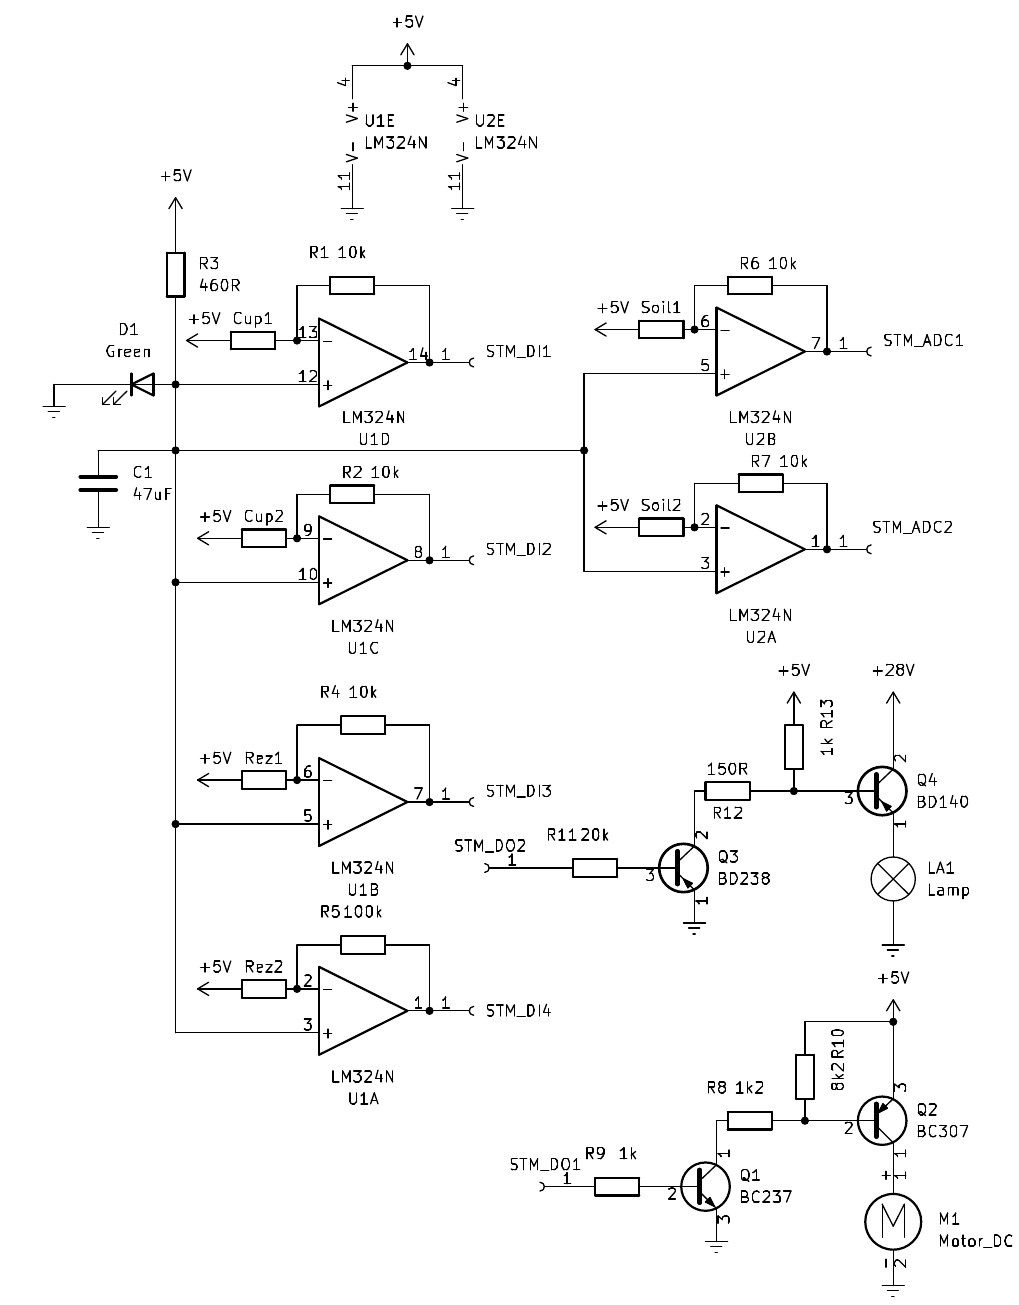
\includegraphics[width=1\linewidth]{schema_pocket.png}
		\caption{Schéma zapojení.}
		\label{fig:schemapocket}
	\end{figure}

	\section{Budoucí vylepšení}
	\subsection{Firmware}
	Při příjmu dat přes sériovou linku může dojít k tomu, že se některá data ztratí. Pokud data přijdou v době, kdy je vykonáván callback sériové linky, data se ztratí. Dále pokud čtu z bufferu uartu a v polovině čtení se změní pomocí callbacku, přijatá data budou znehodnocena. Vyřešit to lze pomocí DMA. To se mi však bohužel nepodařilo včas zprovoznit. DMA jsem dále chtěl využít pro čtení pomocí jednoho převodníku uvnitř procesoru z více pinů tak, že z registrů převodníku jsem data rovnou přesouval do paměti. Zde se mi také nepodařilo DMA uvézt do provozu.
	
	Pro udržení uloženého času uvnitř procesoru lze využít externí baterie a úsporných režimů procesoru. Pro přesnější čas lze také připojit krystal, sloužící čistě pro zdroj reálného času.

	Proces řízení nebude běžet pořád, ale periodicky, aby se šetřila energie a aby v půdě a vodě probíhala ionizace v co nejmenší míře (již implementováno, ale neodzkoušeno).
	
	Funkce pro příjem libovolných datových balíků (již implementováno, ale neodzkoušeno).
	
	Nové zalévací režimy. Například na základě vlhkosti půdy, ale také hlavně na základě času. Například zalévání každé pondělí v danou hodinu.
	
	
	\subsection{Aplikace}
	Pro lepší vizualizaci dat chci v budoucnu prozkoumat knihovnu QWT \cite{bib:swt}, umožňující vložení dalších interaktivních grafických objektů pro technické účely. 
	
	Třída pro kalibraci není úplně dodělaná. Je funkční, ale tlačítko pro umazání poslední hodnoty zatím nefunguje.
	
	Do budoucna se chci také zamyslet nad závislostí vodivosti půdy na její vlhkosti. Nyní je vlhkost určena přímkou, která leží na maximální a minimální hodnotě napětí, které jsem doma experimentálně určil. Z pozorování si však ale myslím, že závislost lineární není. Po nalezení správné závislosti bude také možné vytvořit novou třídu pro kalibraci vlhkosti půdy.	
	
	
	\begin{thebibliography}{9}
		\bibitem{bib:sdcard} kiwih. \emph{cubeide-sd-card} [Online]. [cit. \today]. \newline \url{https://github.com/kiwih/cubeide-sd-card}
			
		\bibitem{bib:sht} henriheimann. \emph{SHT3x} [Online]. [cit. \today]. \newline \url{https://github.com/henriheimann/stm32-hal-sht3x}
		
		\bibitem{bib:dial} Kol. autorů, The Qt Company. \emph{UI Components: Dial Control Example} [Online]. [cit. \today]. \newline \url{https://doc.qt.io/qt-5/qtquick-customitems-dialcontrol-example.html}
		
		\bibitem{bib:mosqq} Kol. autorů, Eclipse Foundation \emph{Eclipse Mosquitto} [Online]. [cit. \today]. \newline \url{https://mosquitto.org/}	
		
		\bibitem{bib:kalibrace} Kol. autorů. \emph{Metoda nejmenších čtverců} [Online]. [cit. \today]. \newline \url{		https://cs.wikipedia.org/wiki/Metoda_nejmen%C5%A1%C3%ADch_%C4%8Dtverc%C5%AF}	
		
		\bibitem{bib:swt} Uwe Rathmann, Josef Wilgen \emph{Qwt - Qt Widgets for Technical Applications} [Online]. [cit. \today]. \newline \url{https://qwt.sourceforge.io/}
		

	\end{thebibliography}
\end{document}